\documentclass[conference]{IEEEtran}
% \IEEEoverridecommandlockouts
% The preceding line is only needed to identify funding in the first footnote. If that is unneeded, please comment it out.
\usepackage{cite}
\usepackage{amsmath,amssymb,amsfonts}
\usepackage{algorithmic}
\usepackage{graphicx}
\usepackage{textcomp}
\usepackage{xcolor}
\usepackage{tikz}
\def\BibTeX{{\rm B\kern-.05em{\sc i\kern-.025em b}\kern-.08em
    T\kern-.1667em\lower.7ex\hbox{E}\kern-.125emX}}

\begin{document}

\title{Invariant Risk Minimization on Score-to-Performance as a Hidden Markov Model}

\author{\IEEEauthorblockN{Quinn Ouyang}
    \IEEEauthorblockA{\textit{School of Music, College of Fine and Applied Arts} \\
        \textit{University of Illinois Urbana-Champaign}\\
        Champaign, Illinois, United States \\
        qouyang3@illinois.edu}
}

\maketitle

\begin{abstract}
    We define score-vs.-performance analysis as a novel task of quantifying how a performance of music compares to its symbolic representation (e.g.\ a recording vs.\ sheet music). One perspective of this task focuses on understanding \textit{how} a musician performs rather than \textit{what} they perform, i.e.\ a ``profile'' of their musical interpretation, style, etc. We propose modeling this as a hidden Markov model where we can directly observe scores and performances, but not performance profiles. Applying invariant risk minimization yields on this chain yields an interpretable representation that minimizes score information.
\end{abstract}

\begin{IEEEkeywords}
    music performance, sheet music, invariant risk minimzation, information theory
\end{IEEEkeywords}

\section{Introduction}
While most audio and music computation research centers around fairly well-defined tasks (e.g\ automatic music transcription or instrument classification), developments on more subjective problems remains scarce. One of the biggest gaps in the field is bridging between symbolic music representations and audio, especially as the academic community tends to seperate these domains into music information retrieval and signal processing, respectively. We take on the challenge of modeling the inherently human process of musical performance.

Fundamentally, scores are manuscripts that represent a musical idea. They usually detail a sequence of pitches (notes) with broad performance directions (instruments, tempos, dynamics, etc.) to interpret and realize as a performance. As musicians inevitably read and play music differently, multiple performances of varying acoustic characteristics can come from a single score. Therefore, through a simplified perspective, a score can map to multiple performances but a performance can map to only one score.

We focus on quantifying musical interpretation, i.e.\ the transition between a music score and a performance of it.


\section{Related Work}

\subsection{Quantifying Musical Expression}

The IEEEtran class file is used to format your paper and style the text. All margins,
column widths, line spaces, and text fonts are prescribed; please do not
alter them. You may note peculiarities. For example, the head margin
measures proportionately more than is customary. This measurement
and others are deliberate, using specifications that anticipate your paper
as one part of the entire proceedings, and not as an independent document.
Please do not revise any of the current designations.

\subsection{Invariant Risk Minimization}
asdihadhadhad

\section{Formulation}

Our goal is to learn a representation of musical expression \(Y\) from paired score-performance data \(X := \{(s_i, p_i)\}_{i=1}^N\). Then we can model this as a simple feed-forward Markov chain \(E \rightarrow X \rightarrow Y \)

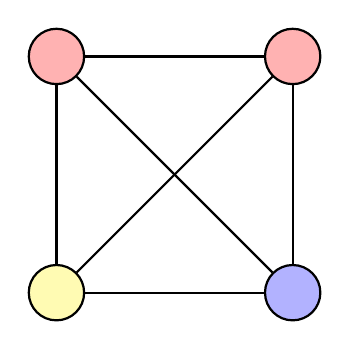
\begin{tikzpicture}[auto, node distance=3cm,
        thick, G node/.style={circle, draw, minimum size=2em}]

    \node[G node, fill=red!30!] (1) {};
    \node[G node, fill=red!30!] (2) [right of=1] {};
    \node[G node, fill=yellow!30!] (3) [below of=1] {};
    \node[G node, fill=blue!30!] (4) [right of=3] {};

    \path
    (1) edge node {} (2)
    (1) edge node {} (3)
    (1) edge node {} (4)
    (2) edge node {} (3)
    (2) edge node {} (4)
    (3) edge node {} (4)
    ;
\end{tikzpicture}

\begin{thebibliography}{00}
    \bibitem{b1} askgdu
\end{thebibliography}
\vspace{12pt}

\end{document}
